\documentclass[11pt, letterpaper, headings=standardclasses]{scrartcl}

\usepackage[margin = 1in]{geometry}

\usepackage{fancyhdr}
	\pagestyle{fancy}
	\fancyhf{}
	\renewcommand{\headrulewidth}{0pt}
	\renewcommand{\footrulewidth}{0pt}
	\lfoot{January 2, 2019}
	\cfoot{\thepage}
	\rfoot{\textsc{Team H}}

\usepackage{tabularx, ltablex, threeparttablex}
	% custom column style
	\newcolumntype{P}{>{\columncolor{LightBlue}\color{White}\raggedright\arraybackslash}l}
	\newcolumntype{C}{>{\centering\arraybackslash}X}
	\newcolumntype{L}{>{\raggedright\arraybackslash}X}

\usepackage{multicol, multirow} % Used for custom table cells

\usepackage{graphicx} % Enables attaching image files

% Custom colors
\usepackage[dvipsnames, table]{xcolor}
	\definecolor{DarkBlue}{HTML}{003554} % Dark blue
	\definecolor{LightBlue}{HTML}{005080} % Light blue

\usepackage[parfill]{parskip}

% mathematics typesetting packages
\usepackage{amssymb, amsmath, mathtools, bbm, xfrac}
	\allowdisplaybreaks
	
\usepackage[colorlinks, allcolors = DarkBlue]{hyperref}

\usepackage{appendix}

\addtokomafont{disposition}{\rmfamily}

\usepackage{tikz}
	\tikzset{
	  headings/base/.style = {
	    outer sep = 0pt,
	    text width = {\textwidth - 0.6666em},
	    align = left,
	    text = white
	  },
	  headings/section/.style = {
	    headings/base,
	    fill = DarkBlue,
	    font = \rmfamily\Large,
	    minimum height = 1cm
	  },
	  headings/subsection/.style = {
	    headings/base,
	    fill = LightBlue,
	    font = \rmfamily\large,
	    minimum height = .8cm
	  }
	}

\newcommand{\colorboxedsec}[2]{%
	\tikz{\node[headings/#1]{#2};}}

\setkomafont{section}{\colorboxedsec{section}}
\setkomafont{subsection}{\colorboxedsec{subsection}}

\usepackage{float}
\usepackage{subcaption}
\usepackage[font={small,it}]{caption}

\begin{document}
	\begin{titlepage}
		\begin{center}
			\vspace*{.5in}
	        
			\Huge
			\textsc{Final Project}
	        
			\Large
			\textsc{Improving Factor-Based Quantitative Investing By Forecasting Company Fundamentals}
			
			\vfill
			
			\normalsize
			\textsc{Team H}
			
			\vfill
			
			Jerry \textsc{Fan} \\
			Rhea Ziran \textsc{Gao} \\
			Casey \textsc{Tirshfield} \\
			Eric \textsc{Wang}
			\vfill
			
			
			January 2, 2019 \\
			IEOR 4720 Deep Learning
					
			\vspace*{.5in}
		\end{center}
	\end{titlepage}
	
	\tableofcontents
	
	\pagebreak
	
	\section{Inspiration}
	The focus of our project is to implement and expand upon the investing strategy presented in the paper, \textit{Improving Factor-Based Quantitative Investing by Forecasting Company Fundamentals}, by John Alberg and Zachary Lipton \cite{paper}. While our methodologies diverge, the fundamental goal remains unchanged---namely, to build a successful portfolio based on a quantitative value investing-like strategy.
	
	Value investing---as opposed to growth investing, for example---relies on the fundamental belief that over a sufficiently long time horizon, a company's market value reflects its intrinsic value, and that the best means by which to predict a company's intrinsic value is to look at its most recently announced fundamental data. The difficulty is that estimating the intrinsic value of a stock is quite challenging.
	
	In an effort to employ technology to address this difficulty, Alberg and Lipton's paper uses deep learning not to predict the current intrinsic value of a stock, but to predict future company fundamentals. They propose that ``the long-term success of an investment should depend on how well-priced the stock currently is with respect to its future fundamentals'' \cite[p. 2]{paper}. They have shown that a portfolio constructed based on clairvoyant knowledge of future fundamentals can drastically outperform the market. Thus, if deep learning can accurately predict future fundamentals, we can use those predictions to construct a highly profitable portfolio. This is the problem that we will expand on in our project.
		
	\section{Data Processing}
	
	\subsection{Acquisition}
	We obtained our data exclusively through University of Pennsylvania's Wharton Research Data Services (WRDS). We pulled quarterly fundamental/market data from the CRSP/Compustat Merged Database.
	
	Our raw data-set was built of the following variables:
	{\footnotesize
	\begin{tabularx}{\textwidth}{P L}
	    \multicolumn{1}{c}{\textbf{Compustat Variable Name}} & \multicolumn{1}{c}{\textbf{Compustat Variable Description}} \\
	    \hline
        CONM & Company Name \\
        TIC & Ticker Symbol \\
        EXCHG & Stock Exchange Code \\
        ACOQ & Current Assets -- Other -- Total \\
        AOQ & Assets -- Other -- Total \\
        APQ & Account Payable/Creditors -- Trade \\
        CHEQ & Cash and Short-Term Investments \\
        COGSQ & Cost of Goods Sold \\
        CSHOQ & Common Shares Outstanding \\
        DLCQ & Debt in Current Liabilities \\
        DLTTQ & Long-Term Debt -- Total \\
        INVTQ & Inventories -- Total \\
        LCOQ & Current Liabilities -- Other -- Total \\
        LTQ & Liabilities -- Total \\
        NIQ & Net Income (Loss) \\
        PPEGTQ & Property, Plant and Equipment -- Total (Gross) -- Quarterly \quad\quad\quad\quad\quad\quad\quad\quad\quad\quad  \\
        RECTQ & Receivables -- Total \\
        REVTQ & Revenue -- Total \\
        TXPQ & Income Taxes Payable \\
        TXTQ & Income Taxes -- Total \\
        XINTQ & Interest and Related Expense -- Total \\
        XSGAQ & Selling, General and Administrative Expenses \\
        CSHTRQ & Common Shares Traded -- Quarter \\
        MKVALTQ & Market Value -- Total \\
        PRCCQ & Price Close -- Quarter \\
        \hline
	\end{tabularx}
	}
	
	Of the variables listed above, our sixteen features were:
	
    {\footnotesize
	\begin{tabularx}{\textwidth}{P L}
	    \multicolumn{1}{c}{\textbf{Feature}} & \multicolumn{1}{c}{\textbf{Compustat Variable Name}} \\
	    \hline
        Revenue & REVTQ \\
        Cost of Goods Sold & COGSQ \\
        Selling, General and Administrative Expenses & XSGAQ \\
        Earnings before interest and taxes & NIQ + TXTQ + XINTQ \quad\quad\quad\quad\quad\quad\quad\quad\quad\quad\quad\quad\quad\quad\quad\quad\quad\quad \\
        Net Income & NIQ \\
        Cash and Short-Term Investments & CHEQ \\
        Receivables & RECTQ  \\
        Inventories & INVTQ \\
        Other Current Assets & ACOQ \\
        Property, Plant and Equipment & PPEGTQ \\
        Other Assets & AOQ \\
        Debt in Current Liabilities & DLCQ \\
        Accounts Payable & APQ \\
        Taxes Payable & TXPQ \\
        Other Current Liabilities & LCOQ \\
        Total Liabilities & LTQ  \\
        \hline
	\end{tabularx}
	}
	
	and our target was:
	
	{\footnotesize
	\begin{tabularx}{\textwidth}{P L}
	    \multicolumn{1}{c}{\textbf{Target}} & \multicolumn{1}{c}{\textbf{Compustat Variable Name}} \\
	    \hline
        EBIT/EV & $\sfrac{\textrm{EBIT} \cdot \textrm{CSHOQ}}{ \textrm{PRCCQ}} + \textrm{DLTTQ} + \textrm{DLCQ} - \textrm{CHEQ}$ \quad\quad\quad\quad\quad\quad\quad\quad\quad\quad\quad\quad\quad\quad\quad\quad\quad\quad\quad\quad\quad\quad\quad\quad \\
        \hline
	\end{tabularx}
	}
	
    \subsection{Cleaning}
    The paper uses all companies from the NYSE, NASDAQ, and AMEX with at least 12 consecutive months of data anytime between 1970 and 2017, with 11815 companies satisfying these criteria. However, upon closer inspection of the selected companies, we found that most of them have very incomplete data. The paper addresses this issue with forward filling. This method is appropriate when NaN values were few and scattered. However, most of the 11815 stocks have consecutive years of missing data for multiple fundamentals; for many stocks over 50\% of the data is missing. It is important to avoid filling time-series data as much as possible because doing so will introduce false step-like patterns, which the deep-learning models will try to learn.
    
    To address the poor quality of data, we introduce stricter rules for stock selection. We consider all stocks from NYSE, NASDAQ, and AMEX with continuous data from January 1990 to present that have at most 6 missing values. Only 100 satisfy these criteria. Though this is a drastic decrease, 100 stocks is enough to achieve the purpose of this project: to explore using deep-learning to predict fundamentals.
    
    \subsection{Processing}
    To prepare our data for input into training, we must first decide how we will model the stocks. More specifically, should we create a new model for each stock or one universal model for all stocks? The paper does not mention which approach they used, but we believe that only the second method is viable. 

    The motivation behind the first approach is that different stocks may exhibit different patterns. While this is likely true, this method is not feasible because each stock has insufficient data to train a deep-learning model. Each stock only contains roughly 30 years of quarterly data, which amounts to less than 100 training samples (70/30 train/test split). For a Basic\_RNN (we will use RNN to refer to the class of neural networks and Basic\_RNN to refer to the basic RNN architecture), the number of training parameters is  
    $$n_{param} = n^2 + kn + nm$$
    Where $n$, $k$, and $m$ are the dimensions of the hidden, output, and input layers. For illustration, let us choose extremely small values for $n,k = 4$. Our input size is 17 (discussed later), so for $n,k,m = 4,4,17$ $n_{param} = 100$. Even for such small $n,k$, we do not have enough samples to train a Basic\_RNN.

    Though the second approach may blur some unique stock dependent patterns, we will have much more data to train our model. This will allow our optimizer to actually find optimal model parameters. Moreover, this will allow for larger networks, which may further increase model performance.

    In order to train a universal model, we must carefully transform the data so that all stocks are comparable to one another. To do so we normalize each stock independently in a for loop. First, we scale the stock's fundamental features by dividing each fundamental by its largest absolute value (some of the fundamental entries are negative). In doing so, we capture the relative changes within each fundamental rather than the absolute changes. This will allow stocks with vastly different fundamental magnitudes to share a model. We also scale the response variable EBIT/EV using largest absolute value. The main advantage of this type of scaling is that it preserves percent changes for each fundamental. 

    After scaling the stock, we reshape its time series data to sequences which will be fed into the neural network. Our goal is to use the past 12 quarters (3 years) to predict next quarter's EBIT/EV value. At any given time, we have the present and historical 16 fundamentals and EBIT/EV values. Thus, the input dimension for our network is is $12\times17$ and our prediction is a single value. After performing normalization and reshaping for each stock, we combine all the sequences into one large dataset.
    
	\section{Modelling}
	\subsection{Linear Regression}
	The baseline model for comparison purposes is Multiple Linear Regression. This is the benchmark that the paper uses to gauge the efficacy of neural network models. However, the paper does not describe what the inputs for the regression are. We believe there are two likely options. First, the authors might have used the current 16 fundamentals and EBIT/EV to predict the future EBIT/EV. However, this does not capture any time-dependency in the data. The second, and more likely option, is to regress solely on historical EBIT/EV; the response is a linear combination of past EBIT/EV values. More specifically $y_1 = k + \sum^{0}_{-11} \beta_i \times y_i$ where the $y=\text{EBIT/EV}$ and the subscript represents quarters from present. We use the latter regressions approach to train our model.
	
	\begin{figure}[H]
    \centering
    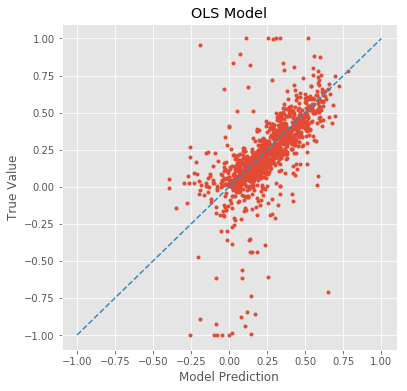
\includegraphics[width=0.6\textwidth]{ols_plot.png}
    \end{figure}
	
	Since the OLS model is a linear combination of past values, it captures the general trend of the historical values. This seems to perform moderately well, as shown by the clustering of points along $y=x$. The testing MSE and MAE are respectively $0.0330$ and $0.1018$ and the $R^2 = 0.5464$.
	
	\subsection{Deep Neural Networks}
	We will use recurrent neural networks to try to better model the evolution of EBIT/EV. Since we will use the past 12 quarters of data to forecast one quarter into the future, our RNNs will have 12 cells. To determine the best architectures of the RNN, we will perform a grid-search over difference possible architecture combinations. We will first test Basic\_RNN/GRU/LSTM, hidden state sizes $16,32,64,128$, and network depths $1,2,3$. By network depth $n$, we mean an $n$ stacked RNN. We will use $\texttt{batch size}=4$ and $\texttt{epochs}=200$, these two parameters will be further tuned after we've determined the best architectures. The table below summarizes the results of our search.

	\begin{figure}[H]
    \centering
        \begin{subfigure}{.33\textwidth}
      \centering
      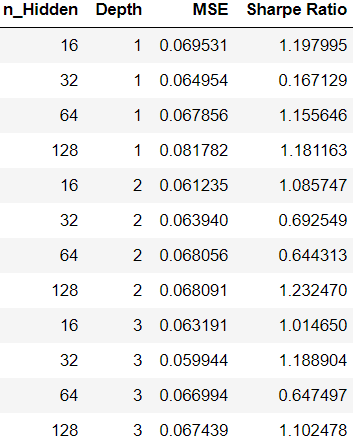
\includegraphics[width=.9\linewidth]{RNN.png}
      \caption{Basic\_RNN}
      \label{fig:sub1}
    \end{subfigure}%
    \begin{subfigure}{.33\textwidth}
      \centering
      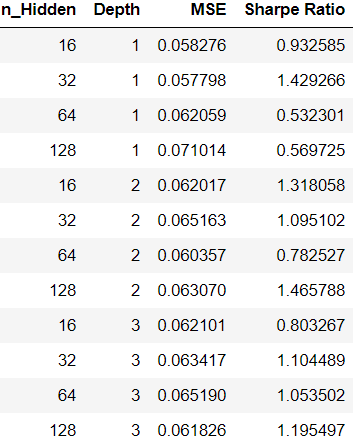
\includegraphics[width=.9\linewidth]{GRU.png}
      \caption{GRU}
      \label{fig:sub1}
    \end{subfigure}%
    \begin{subfigure}{.33\textwidth}
      \centering
      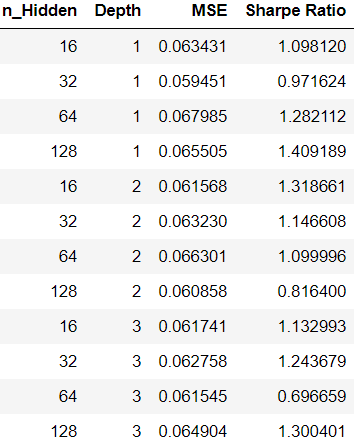
\includegraphics[width=.9\linewidth]{LSTM.png}
      \caption{LSTM}
      \label{fig:sub2}
    \end{subfigure}
    \caption{Performance of various RNN architectures. MSE refers to testing mean squared error and Sharpe Ratio refers to the performance of the portfolio constructed based on the model output. We will discuss this in more detail later.}
    \label{fig:test}
    \end{figure}
    
	From the search, we can see that the Basic\_RNN favors larger networks while GRU/LSTM favor simpler networks (in terms of hidden size and depth). This observation was made by grouping the results by depth or hidden size. We believe this to be the case because Basic\_RNN is inherently simpler than GRU/LSTM. Thus, Basic\_RNN requires additional hidden size/depth to capture the same patterns as GRU/LSTM.

	We believe that we should typically shy away from larger networks because we do have a tremendous amount of data; we only have $\sim3000$ training samples. When we work with large networks such as $\texttt{depth}=3$ and $\texttt{n\_hidden}=128$, we simply do not have enough data to adequately train these models. Due to our data limitations, we should focus on smaller networks.

	Though our deep learning models certainly have predictive power, none of the architectures so far have outperformed our baseline OLS. The efficacy of our OLS model inspired us to add basic attention to our networks. The rationale being that basic attention will take a weighted average of historical hidden states just like how OLS simply takes a weighted average of historical values. We hoped that adding can increase our reduce the testing MSE while simultaneously improving portfolio performance. We run the same search as before but now we add an attention layer on top of the RNN.

	\begin{figure}[H]
    \centering
        \begin{subfigure}{.33\textwidth}
      \centering
      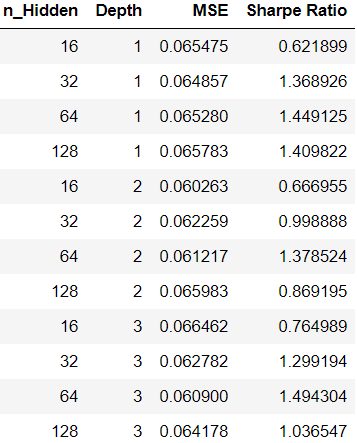
\includegraphics[width=.9\linewidth]{RNN_att.png}
      \caption{Basic\_RNN}
      \label{fig:sub1}
    \end{subfigure}%
    \begin{subfigure}{.33\textwidth}
      \centering
      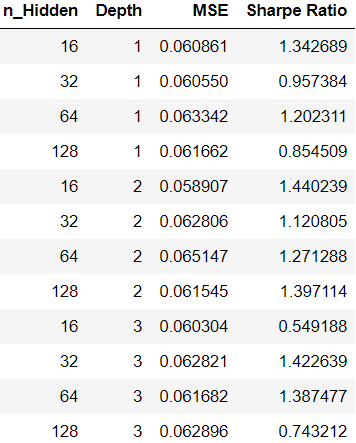
\includegraphics[width=.9\linewidth]{GRU_att.png}
      \caption{GRU}
      \label{fig:sub1}
    \end{subfigure}%
    \begin{subfigure}{.33\textwidth}
      \centering
      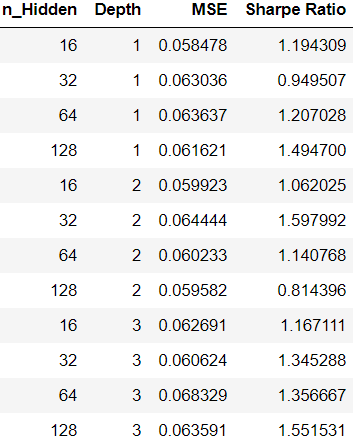
\includegraphics[width=.9\linewidth]{LSTM_att.png}
      \caption{LSTM}
      \label{fig:sub2}
    \end{subfigure}
    \caption{Performance of various Attention RNN architectures.}
    \label{fig:test}
    \end{figure}
	
	Once again, we notice that RNN attention architectures favor larger networks while GRU/LSTM favor smaller networks. Morevoer, we notice that adding attention improved both the MSE and Sharpe Ratio in most cases. To better visualize the improvement of attention, we average the performances different architecture classes.
	
	{\footnotesize
	\begin{tabularx}{\linewidth}{P c | c | c | c}
	\cellcolor{white} & \multicolumn{2}{c}{\textbf{Attention}} & \multicolumn{2}{c}{\textbf{No Attention}}\\
    \multirow{-2}{*}{\cellcolor{white}\color{black}\textbf{Cell Type}} & \multicolumn{1}{c}{\textbf{MSE}} & \multicolumn{1}{c}{\textbf{Sharpe}} & \multicolumn{1}{c}{\textbf{MSE}} & \multicolumn{1}{c}{\textbf{Sharpe}}\\
    \cline{2-5}
    Basic\_RNN & 0.0638 & 1.1132 & 0.0669 & 0.9425\\
    GRU & 0.0619 & 1.1407 & 0.0627 & 1.0235\\
    LSTM & 0.0622 & 1.2401 & 0.0633 & 1.1264\\
    \hline
    \end{tabularx}
    }
    
    Based on these observations, we selected several candidate architectures for further tuning. Since, GRU/LSTM outperform Basic\_RNN significantly, we will focus on GRU/LSTM models. For these models, we determined that smaller networks are more feasible given our data and more favorable in terms of performance. Thus, we will only further tune GRU/LSTM $\texttt{depth}=1$ $\texttt{n\_hidden}=16$, $\texttt{depth}=1$ $\texttt{n\_hidden}=32$, and $\texttt{depth}=2$ $\texttt{n\_hidden}=16$. For this tuning we will adjust $\texttt{epochs}=100,150,200,250,300,$ $\texttt{batch size}=4,8,16$ and $\texttt{learning rate}=0.0001,0.001,0.01,0.1$. The top 5 models with the lowest MSE are: 
    
    \begin{figure}[H]
    \centering
    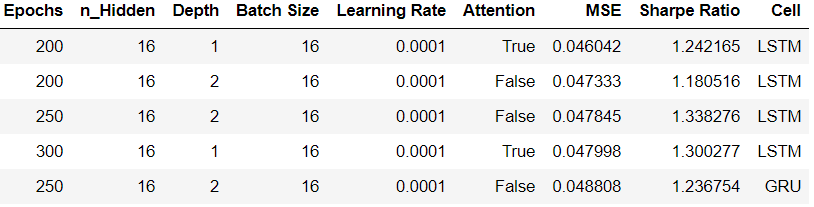
\includegraphics[width=0.7\textwidth]{best_models.png}
    \end{figure}
	
	Interestingly, all the best performing models all use $\texttt{batch size}=16$ and $\texttt{learning rate}=0.0001$. When attention is used a single layer RNN is best. When there is no attention, a double layer RNN is best. Since top model has a significantly smaller MSE than the other models, it is the final product of our modelling. Thus, our final model is Attention LSTM with $\texttt{depth}=1$ and $\texttt{n\_hidden}=16$, trained with $\texttt{epoch}=200$, $\texttt{batch size}=16$ and $\texttt{learning rate}=0.0001$.
	
	\section{Final Model}
	
	\subsection{Performance}
    To better understand what our model actually does, we compared its predictions to the testing set's true values.
    \begin{figure}[H]
    \centering
    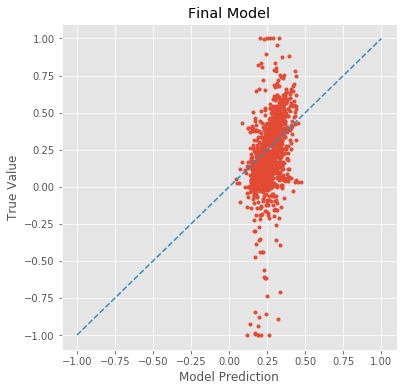
\includegraphics[width=0.6\textwidth]{final_model_predictions.png}
    \end{figure}
    It's clear that our model's predictions are much less variable than the true values. Our predictions have $\texttt{mean}=0.258$ and $\texttt{std}=0.072$, whereas the true values have $\texttt{mean}=0.199$ and $\texttt{std}=0.258$. The discrepancy between the model and the true values can be visualized clearly using the histogram below. 
    \begin{figure}[H]
    \centering
    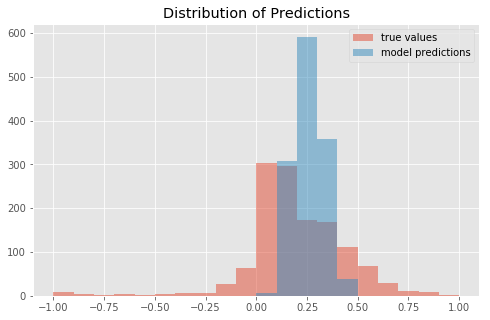
\includegraphics[width=0.7\textwidth]{dist_predictions.png}
    \end{figure}
    The histogram confirms that our model is not only biased, but does not adequately capture the variability in the data, just as. Finally, let us look at some stocks individually to further understand how our model behaves. 
    \begin{figure}[H]
    \centering
        \begin{subfigure}{.33\textwidth}
      \centering
      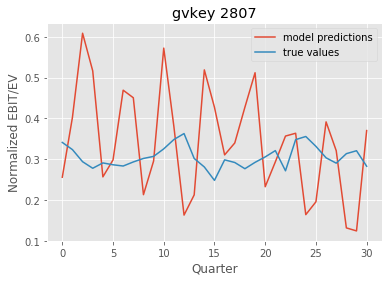
\includegraphics[width=1\linewidth]{stock1.png}
    \end{subfigure}%
    \begin{subfigure}{.33\textwidth}
      \centering
      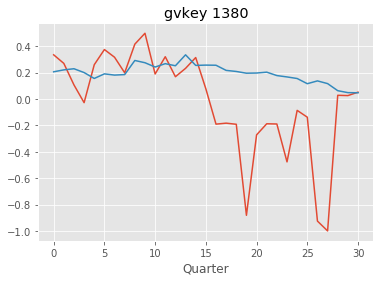
\includegraphics[width=1\linewidth]{stock2.png}
    \end{subfigure}%
    \begin{subfigure}{.33\textwidth}
      \centering
      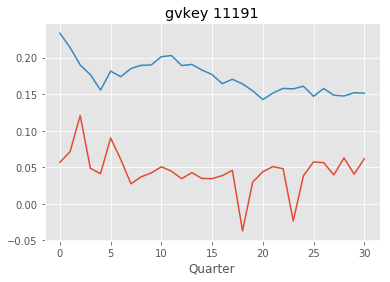
\includegraphics[width=1\linewidth]{stock3.png}
    \end{subfigure}
    \caption{Model predictions for three stocks. gvkey is an unique stock identifier.}
    \label{fig:test}
    \end{figure}
    
    In the first subplot, we can clearly see how our model does capture the variability in the data. In the second subplot, we see that our model recognizes the drop in EBIT/EV after quarter 15 by trending downwards. However, it is once again unable to capture the severity of the drop due to its invariability. In the last subplot, we see that our model completely misses the mark. This is due to the fact that our model almost always predicts values near the mean of 0.258. Thus, when the true EBIT/EV values are far from 0.258, our model fails.
    
    \subsection{Explanation of Model Shortcomings and Possible Solution}
    As mentioned previously, our model was not only biased but also did not adequately capture the variability of EBIT/EV. In fact, a simple OLS using the historical EBIT/EV beat our best model. Theoretically, our attention LSTM should be at least as good as OLS; its architecture can replicate OLS, but can also capture more complex dependencies.
    
    We believe that the reason for our model's shortcomings is that there are too many inputs and not enough data. Many of the input fundamentals are likely redundant. When these features are included in the model, they increase the number of parameters that need to be trained without adding much to the model. If we had infinite data, our optimizer should eventually be able to determine that these extraneous features are useful and assign them very little weights. However, we only have around 3000 training samples, which is likely not enough for the model to learn what is important and distinguish all the extraneous features. 
    
    Since, the data source is rather low quality, it will be difficult to obtain a tremendous amount of data. Thus, we believe that feature selection is a more practical remedy this problem. Perhaps, one could start with a simple attention/no attention LSTM using only historical EBIT/EV as inputs (input vector length 1). Then one can add an additional fundamental (input vector length 2) to see if the model performance increase. After determining the best second fundamental, one can try to add a third (input vector length 3). One can repeat this until model performance stops improving. This method is exactly like forward-selection for multiple regression. We hope that this will reduce the input vector dimension to only include salient features.
    
    Of course, we should still try to obtain more data. Our standards for data were quite high. By reducing the requirement, one could likely double or even triple the number of training/testing samples. However, one must be careful when relaxing data requirements as it could lead to bad data, which could undermine the benefits of more data.
    
    \subsection{Portfolio}
    The trading strategy proposed by Alberg and Lipton is to hold the stocks with the highest EBIT/EV. Our model predicted normalized EBIT/EV, which we can easily transform back to EBIT/EV. Since we used far fewer stocks than Alberg and Lipton, we will divide our portfolio resources into only 100 stocks. The performance of our portfolio in the testing period is plotted below.
    
    \begin{figure}[H]
    \centering
    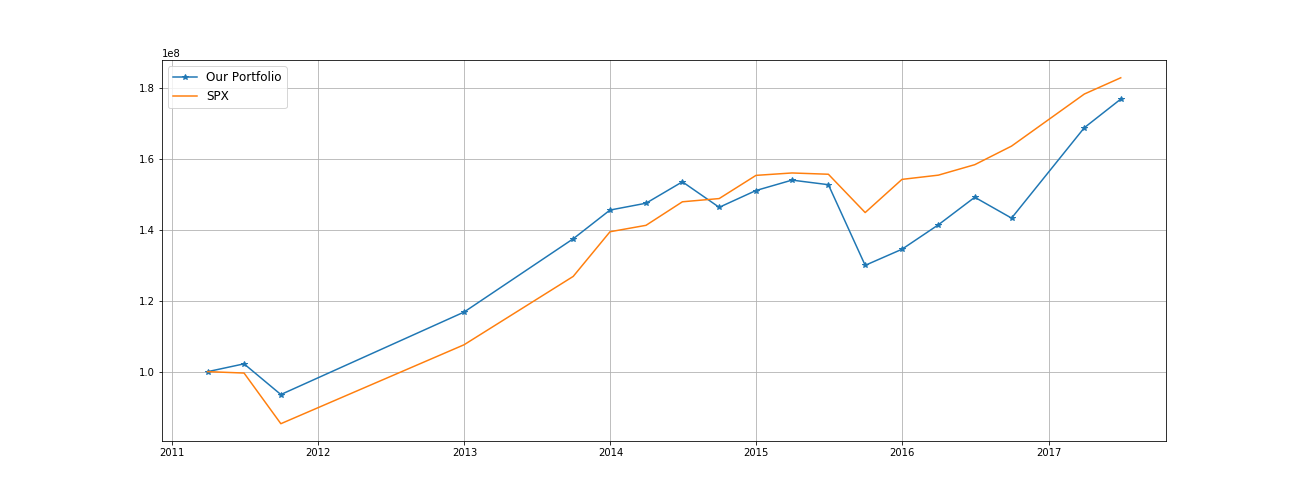
\includegraphics[width=1\textwidth]{portfolio.png}
    \end{figure}
    
    As we can see, our portfolio roughly follows the S\&P500. The purpose of aim of our project is to use deep learning to predict time-series of fundamental data, not necessarily constructing the most profitable portfolio. Thus, we will not worry too much about the performance of the portfolio. We have implemented the algorithm so that an user can satisfy his/her curiosity and check the portfolio's performance. 
    
	\section{Conclusion}
	Inspired by Alberg and Lipton, our group attempted to utilize deep learning to forecast future EBIT/EV ratio. Because of our strict data requirements, our data-set was much smaller than that used by Alberg and Lipton. Morevoer, our data processing differed significantly from Alberg and Lipton because our goal was to train an universal model that was independent of the individual stock. We tested a variety of architectures and found that smaller networks performed better. Our final model is Attention LSTM with $\texttt{depth}=1$, $\texttt{n\_hidden}=16$, trained with $\texttt{epoch}=200$ $\texttt{batch size}=16$ $\texttt{learning rate}=0.0001$. However, even our best model could not outperform OLS with only historical EBIT/EV values. We believe that the source of our model's shortcoming is the redundancy of many input features, which is particularly problematic because our data-set is rather limited. The next step in this endeavor would be to perform feature selection; forward-selection starting with only historical EBIT/EV as inputs would be a good approach. Finally, we have implemented the trading algorithm proposed by Alberg and Lipton which allows us to use our forecast of EBIT/EV to construct and rebalance a portfolio. 
	
	\begin{appendices}
		\section{Codebase}
			Our project's codebase can be found in the following \href{https://github.com/caseytirshfield/deeplearninveststrat}{GitHub Repository}.
	\end{appendices}
	
	\pagebreak
	
	\bibliographystyle{unsrt}
	\bibliography{references.bib}
\end{document}